
\section{NLO Monte Carlo event generators\protect\footnote{M. Felcini, F. Krauss, 
F. Maltoni, P. Nason and J. Yu.}}
\newcommand\pperpmin{p_\perp^{\rm min}}

\def\fortran{Fortran\xspace}
%\def\pythia{Pythia\xspace}
\providecommand{\pythia}{{\sc Pythia}}
\def\phojet{Phojet\xspace}
%\def\pythiasix{Pythia~6\xspace}
\providecommand{\pythiasix}{{\sc Pythia~6}}
%\def\pythiaeight{Pythia~8\xspace}
\providecommand{\pythiaeight}{{\sc Pythia~8}}
%\def\herwig{Herwig\xspace}
\providecommand{\herwig}{{\sc Herwig}}
%\def\herwigsix{Herwig~6\xspace}
\providecommand{\herwigsix}{{\sc Herwig~6}}
%\def\herwigpp{Herwig\raisebox{0.1ex}{\small $++$}\xspace}
\providecommand{\herwigpp}{{\sc Herwig}\raisebox{0.1ex}{\small $++$}}
%\def\sherpa{Sherpa\xspace}
\providecommand{\sherpa}{{\sc Sherpa}}
%\def\alpgen{AlpGen\xspace}
\providecommand{\alpgen}{{\sc AlpGen}}
\def\helac{HELAC\xspace}
\def\charybdis{Charybdis\xspace}
\def\jimmy{Jimmy\xspace}
\def\rivet{Rivet\xspace}
\def\rivetgun{Rivetgun\xspace}
\def\professor{Professor\xspace}
\def\fastjet{FastJet\xspace}
\def\hepmc{HepMC\xspace}
\def\agile{AGILe\xspace}
\def\hztool{HZTool\xspace}
\def\numpy{NumPy\xspace}
\def\scipy{SciPy\xspace}
\def\minuit{Minuit\xspace}
\def\pyminuit{PyMinuit\xspace}
\def\python{Python\xspace}
\def\kT{\ensuremath{k_{\mathrm{T}}}} % Subscript roman not italic (EE)
%--
%\newcommand\POWHEG{{P\scalebox{0.9}{OWHEG}}\xspace}
\newcommand\POWHEG{{\sc P\scalebox{0.9}{OWHEG}}\xspace}
\newcommand\POWHEGBOX{{\sc P\scalebox{0.9}{OWHEG} B\scalebox{0.9}{OX}}\xspace}
\newcommand\MCatNLO{{\sc M\scalebox{0.9}{C}@N\scalebox{0.9}{LO}}\xspace}
%\newcommand\MCatNLO{\tt MC@NLO}
\newcommand\ARIADNE{{\sc A\scalebox{0.9}{RIADNE}}\xspace}
\newcommand\ADICIC{{\sc A\scalebox{0.9}{DICIC}++}\xspace}
\newcommand\AMEGIC{{\sc A\scalebox{0.9}{MEGIC}++}\xspace}
\newcommand\Comix{{\sc Comix}\xspace}
\newcommand\HNNLO{{\sc H\scalebox{0.9}{NNLO}}\xspace}
\newcommand\MGME{{\sc M\scalebox{0.9}{AD}G\scalebox{0.9}{RAPH/}M\scalebox{0.9}{AD}E\scalebox{0.9}{VENT}}\xspace}

%\title{\centerline{Accurate MonteCarlo's for Higgs Physics at the LHC}}

%\author{M.~Felcini$^1$, F. Krauss$^5$, F.~Maltoni$^2$, P.~Nason$^3$, J.~Yu$^4$}

%\vskip.5cm

%\institute{$^1$ University College Dublin, School of Physics, Ireland.
%\\$^2$ Centre for Cosmology, Particle Physics and Phenomenology (CP3), Louvain-la-Neuve, Belgium
%\\$^3$ Universit\`a di Milano-Bicocca, 20126 Milano, Italy.
%\\$^4$ Department of Physics, University of Texas at Arlington, Texas, US.}

%\maketitle

%\begin{abstract}
%We briefly present the basic principles of Monte Carlo's at NLO and with matrix
%element merging and the state-of-the-art tools available for accurate 
%Higgs production processes at the LHC.
%\end{abstract}

%\setcounter{tocdepth}{1}
%\tableofcontents
%\setcounter{footnote}{0}

%%%%%%%%%%%%%%%%%%%%%%%%%%%%%PART%%%%%%%%%%%%%%%%%%%%%%%%%%%%%

%%%%%%%%%%%%%%%%%%%%%%%%%%%%%PART%%%%%%%%%%%%%%%%%%%%%%%%%%%%%

%%%%%%%%%%%%%%%%%%%%%%%%%%%%%%%%%%%%%%%%%%%%%%%%%%%%%%%%%%%%%%%%%%%%%%%%%%%%%

\subsection{Introduction}

In recent years Monte Carlo event generators have been the subject of great
theoretical and practical developments, most significantly in the extension
of existing parton-shower simulations to consistently include exact
next-to-leading order (NLO) corrections~\cite{Frixione:2002ik,
Frixione:2003ei,Frixione:2005vw,Frixione:2006gn,Frixione:2007zp,Frixione:2008yi,
LatundeDada:2007jg,Nason:2004rx,Nason:2006hfa,Frixione:2007nu,Frixione:2007vw,
Frixione:2007nw,LatundeDada:2006gx,Hamilton:2008pd,Hamilton:2009za,
Alioli:2008gx,Alioli:2008tz,Alioli:2009je,LatundeDada:2008bv}  
%\cite{Frixione:2003ei},
%\cite{Frixione:2005vw},
%\cite{Frixione:2006gn},
%\cite{Frixione:2007zp},
%\cite{Frixione:2008yi},
%\cite{LatundeDada:2007jg},
%\cite{Nason:2004rx},
%\cite{Nason:2006hfa},
%\cite{Frixione:2007nu},
%\cite{Frixione:2007vw},
%\cite{Frixione:2007nw},
%\cite{LatundeDada:2006gx},
%\cite{Hamilton:2008pd},
%\cite{Hamilton:2009za},
%\cite{Alioli:2008gx},
%\cite{Alioli:2008tz},
%\cite{Alioli:2009je},
%\cite{LatundeDada:2008bv}  
and, separately, in the consistent combination of parton-shower simulations 
and high-multiplicity tree-level matrix-element generators~%
\cite{Mangano:2001xp,Catani:2001cc,Lonnblad:2001iq,Krauss:2002up,
Mrenna:2003if,Schalicke:2005nv,Alwall:2007fs,Hoeche:2009rj,Hamilton:2009ne}.  
%\cite{Catani:2001cc},
%\cite{Lonnblad:2001iq},
%\cite{Krauss:2002up},
%\cite{Mrenna:2003if},
%\cite{Schalicke:2005nv},
%\cite{Alwall:2007fs},
%\cite{Hoeche:2009rj},
%\cite{Hamilton:2009ne}.  

In this note we aim at concisely reviewing the basic principles of the new 
generation of tools which are now available, underlying the most important 
improvements with respect to a more standard parton-shower approach.  We 
provide also guidelines for experimentalists on which tools to use for a 
given Higgs production channel, on the possible improvements/limitations and 
on how to perform a meaningful cross validation of the MC tools used in an 
experimental analysis vis-a-vis the best theoretical predictions available 
at a given moment (for example, at NNLO level).  As a result, we provide 
enough motivation for the new MC tools to be used as {\em default} analysis 
tools, both to better tune Higgs-boson searches and to perform precise 
measurements of its properties.  We also aim at providing guidelines for
how and when to use these tools.  We conclude by summarising the results 
and by commenting on the readiness of these theoretical tools for 
anticipated 
Higgs analyses, and by adding a wish-list for tools from the experimentalist 
point of view.   

\subsection{Embedding higher-order corrections into parton-shower
  Monte Carlo event generators}
\subsubsection{NLO cross sections}

Let us start by reminding the equation describing the calculation of 
next-to-leading order corrections in QCD for a $2\to n$ process; 
schematically it reads
\begin{equation}\label{eq:nlocorr}
{\rm d}\sigma^{\rm (NLO)}
=
{\rm d}\Phi_B\left[B(\Phi_B)+V(\Phi_B)\right]+
{\rm d}\Phi_R R(\Phi_R)\,,
\end{equation}
where $\Phi_B$ and $\Phi_R$ denote the phase-space elements related to the
$2\to n$ (Born level) and $2\to n+1$ (real-emission correction) kinematics;
$B(\Phi_B)$, $V(\Phi_B)$ denote the Born-level and the virtual contribution, 
while $R(\Phi_R)$ is the real-emission correction.

In this equation the virtual term contains soft and collinear divergences.
When integrated over the full real phase space, the real term generates 
soft and collinear divergences, too, and only when {\em infrared(IR)-safe} 
quantities are computed, these divergences cancel to yield a finite result.
IR-safe observables $O(\Phi)$ can be best understood by considering
the soft or collinear limit of $\Phi_R$, i.e.\ when the additional parton
has low energy or is parallel to another parton.  In this
limit, an IR-safe observable yields $\lim O(\Phi_R)=O(\Phi_B)$, where the 
Born-level configuration $\Phi_B$ is obtained from $\Phi_R$ by eliminating 
the soft particle (in case of soft singularities) or by merging the collinear 
particles (in case of collinear singularities).

Technically, singularities are often handled with the subtraction method, 
where the real phase space is parametrized in terms of an underlying Born 
phase space $\Phi_B$ and a radiation phase space $\Phi_{R|B}$. The only 
requirement upon this parametrization is that, in the singular limits, by 
merging collinear partons, or eliminating the soft parton, the real phase 
becomes equal to the underlying Born one.  Then the expectation value of
an IR-safe observable reads
\begin{eqnarray}
\int {\rm d}\sigma^{\rm (NLO)} O(\Phi)&=&
\int {\rm d}\Phi_B\left[B(\Phi_B)+V(\Phi_B)\right]O(\Phi_B)
+\int {\rm d}\Phi_R R(\Phi_R)\; O(\Phi_R)
\nonumber \\
&=&\int {\rm d}\Phi_B\left[B(\Phi_B)+V(\Phi_B)
+\int {\rm d}\Phi_{R|B}S(\Phi_R)\right]O(\Phi_B)
\nonumber \\
&+&\int {\rm d}\Phi_R \left[R(\Phi_R)\; O(\Phi_R)-S(\Phi_R)
O(\Phi_B)\right]\;. \label{eq:subtractionmethod}
\end{eqnarray}
The third member of the above equation is obtained by adding and subtracting
the same quantity from the two terms of the second member.  The terms 
$S(\Phi_{R|B})$ are the subtraction terms, which contain all soft and collinear 
singularities of the real-emission term.  Typically, using the universality 
of soft and collinear divergences, they are written in a factorised form as
\begin{equation}
    S(\Phi_R) = B(\Phi_B)\otimes \tilde S(\Phi_{R|B})\,,
\end{equation}  
where the $\tilde S(\Phi_{R|B})$ can be composed from universal, 
process-independent subtraction kernels with analytically known (divergent) 
integrals.  These integral, when summed and added to the virtual term, yield 
a finite result.  The second term of the last member of 
Eq.\,(\ref{eq:subtractionmethod}) is also finite if $O$ is an IR-safe 
observable, since by construction $S$ cancels all singularities in $R$ in 
the soft and collinear regions.

In the following we will always write the NLO corrections in the form
of Eq.\,(\ref{eq:nlocorr}), assuming that a subtraction procedure is
carried out in order to evaluate it explicitly.

\subsubsection{Parton shower (PS)}
Parton showers are able to dress a given Born process with all the dominant
(i.e.\ enhanced by collinear logarithms, and to some extent also soft ones)
QCD radiation processes at all orders in perturbation theory.
In particular, also the hardest radiation includes next-to-leading order
corrections, but only the dominant ones, i.e.\ those
given by the leading logarithms.
The cross section for the hardest emission in a shower -- often this is the 
first emission -- reads:
\begin{equation}
\label{Eq:1storder_in_PS}
{\rm d}\sigma^{\rm PS} = 
{\rm d}\Phi_B B(\Phi_B)
\left[\Delta(\pperpmin) + 
      {\rm d}\Phi_{R|B} \Delta(\pT(\Phi_{R|B}))
\frac{R^{\rm PS}(\Phi_R)}{B(\Phi_B)}   \right]\,,
\end{equation}
where $\Delta(\pT)$ denotes the Sudakov form factor
\begin{equation}
\Delta(\pT) = 
\exp\left[-\int\,{\rm d}\Phi_{R|B}\frac{R^{\rm PS}(\Phi_R)}{B(\Phi_B)} 
\Theta(\pT(\Phi_{R})-\pT)\right]\;.
\end{equation}
This Sudakov form factor can be understood as a no-emission probability
of secondary partons down to a resolution scale of $\pT$.
Here $R^{\rm PS}$ represents the PS approximation to the real cross section,
typically given schematically by a product of the underlying Born-level
term folded with a process-independent universal splitting function $P$:
\begin{equation}
R^{\rm PS}(\Phi)=P(\Phi_{R|B})\,B(\Phi_B).
\end{equation}
In this framework, $\Phi_{R|B}$ is often expressed in terms of three showering 
variables, like the virtuality $t$ in the splitting process\footnote{
           In more modern parton showers the transverse momentum
           of the splitting or the (scaled) opening angle serve
           as ordering variables instead of the virtuality, such
           a choice usually allows to catch more of the leading
           logarithmic terms.
}, the energy fraction of the splitting $z$ and the azimuth $\phi$.
The above definition of the Sudakov form factor, guarantees
that the square bracket in Eq.\ (\ref{Eq:1storder_in_PS}) integrates to unity,
a manifestation of the probabilistic nature of the parton shower.
Thus, integrating the shower cross section over the radiation variables
yields the total cross section, given at LO by the Born amplitude.
The corresponding radiation pattern consists of two parts: one 
given by the first term in the square bracket, where no further resolvable 
emission above the parton-shower cut-off $\pperpmin$ -- typically of the order
of $1$\UGeV\ -- emerges, and the other given by the second term in the square bracket describing the first emission, as determined by the splitting kernel.

It is important to stress that the real-emission cross section in a PS 
generator is only correct in the small angle and/or soft limit, where
$R^{\rm PS}$ is a reliable approximation of the complete matrix element.

While rather crude, the PS approximation is a very powerful one, due mainly
to the great flexibility and simplicity in the implementation of
 $2 \to 1$ and $2\to 2$ high-$Q^2$ processes. In addition, once 
augmented with a hadronisation model the simulation can easily provide a 
full description of a collision in terms of physical final states, i.e., 
hadrons, leptons and photons.  In the current terminology a generic Monte 
Carlo generator mainly refers to such tools, the most relevant examples of are 
\pythiasix\ and \pythiaeight~\cite{Sjostrand:2006za,Sjostrand:2007gs}, 
\herwig~\cite{Corcella:2000bw}, \herwigpp~\cite{Bahr:2008pv}, and 
\sherpa~\cite{Gleisberg:2003xi}.  

It should be noted here, however, that each of these tools employs a 
variety of the more advanced methods listed below, to enhance its accuracy 
in the description of the radiation pattern or the total cross sections,
thus going in some cases beyond the simple PS approach.


\subsubsection{Matrix-element correction (MEC)}
\label{mec}
A first improvement of the parton-shower approximation is to correct
the hardest emission with the
{\em exact first-order real-emission matrix element}.
This has traditionally been achieved by matrix-element corrections%
~\cite{Bengtsson:1986hr,Gustafson:1987rq,Seymour:1994we,
Seymour:1994df,Miu:1998ju,Lonnblad:1995ex}. 
%\cite{Gustafson:1987rq},
%\cite{Seymour:1994we},
%\cite{Seymour:1994df},
%\cite{Miu:1998ju},
%\cite{Lonnblad:1995ex}. 
These are provided by either replacing the approximate expression for the 
real-emission cross section $R^{\rm PS}$ with the exact one $R$, or by adding 
real-emission events with a cross section $R-R^{\rm PS}$, in order to 
compensate for the PS inaccuracies (including lack of complete coverage of 
phase space) in large-angle emissions.  Matrix-element corrections in PS 
have only been introduced for the most simple processes, such as Drell--Yan or
$\PW$ production, Higgs production in gluon fusion, or top decay, all
present in \pythiasix, \pythiaeight, \herwig, and \herwigpp.  

Decomposing the real-emission cross section into a singular and non-singular 
part, $R=R^{s}+R^{f}$ (both being non-negative), the first-emission 
cross section in this method can be written as
\begin{equation}\label{Eq:MEC}
{\rm d}\sigma^{\rm MEC} =
{\rm d}\Phi_B B(\Phi_B)
\left[\bar\Delta(\pperpmin)+\int\limits_{\pperpmin}{\rm d}\Phi_{R|B}
      \frac{R^{s}(\Phi_R)}{B(\Phi_B)}
      \bar\Delta(\pT(\Phi_{R|B}))\right]
+ {\rm d}\Phi_R R^{f}(\Phi_R)\,,
\end{equation}
where the modified Sudakov form factor is given by replacing the splitting 
function with the ratio of real-emission and Born-level matrix elements,
\begin{equation}
\bar \Delta(\pT) = 
\exp\left[-\int\limits_{\pperpmin}{\rm d}\Phi_{R|B}
  \frac{R^{s}(\Phi_R)}{B(\Phi_B)}\right]\,.
\end{equation}
Note that the term in the square bracket integrates to unity,
as in the usual PS case.  In the \pythia\ implementation $R^{f}=0$, while in \herwig, due to 
the lack of full phase-space coverage the term $R^{f}$ is introduced, with 
support only in the region of phase space that the parton shower cannot fill.
In the latter the hardest emission is not necessarily the first one,
since the ordering parameter is the splitting angle.
The correction is thus applied
to all branchings that are the hardest so far in the shower development.

While this method correctly reproduces the first-emission kinematics (formally
this is a next-to-leading order effect with respect to the Born-level 
cross section), 
it does not include the full next-to-leading order accuracy to the total 
cross section.


\subsubsection{NLO+PS}
\label{nlops}
Several proposals have been made for the full inclusion of complete NLO 
effects in PS generators. At this moment, only two of them have reached a
mature enough stage to be used in practice: \MCatNLO~\cite{Frixione:2002ik} and 
\POWHEG~\cite{Nason:2004rx}.  Both methods correct -- in different ways -- 
the real-emission matrix element to achieve an exact tree-level emission 
matrix element, even at large angle.  As we have seen in the previous 
subsection, this is what is also achieved with matrix-element corrections in 
parton showers, at least for the simplest processes listed earlier.  This, 
however, is not sufficient for the NLO accuracy, since the effect of 
virtual corrections also needs to be included.  In both methods, the real-emission 
cross section is split into a singular and non-singular part,
$R=R^{s}+R^{f}$.  One then computes the total NLO inclusive cross 
section, excluding the finite contribution, at fixed underlying Born 
kinematics, defined as
\begin{equation}\label{eq:nlocorr1}
\bar{B}^{s}=B(\Phi_B)+\left[V(\Phi_B)+
\int{\rm d}\Phi_{R|B} R^{s}(\Phi_{R|B})\right]\,,
\end{equation}
and uses the formula
\begin{equation}
\label{Eq:Powheg}
{\rm d}\sigma^{\rm NLO+PS} =
{\rm d}\Phi_B\bar B^{s}(\Phi_B)
\left[\Delta^s(\pperpmin) 
  +  {\rm d}\Phi_{R|B}
      \frac{R^{s}(\Phi_R)}{B(\Phi_B)}
      \Delta^s(\pT(\Phi))\right] 
+ {\rm d}\Phi_R R^{f}(\Phi_R)
\end{equation}
for the generation of the events.  In this formula, the term $\bar B$ can be 
understood as a local $K$-factor reweighting the soft matrix-element 
correction part of the simulation.  Clearly, employing the fact that 
the term in the first square bracket integrates to unity, as before, the 
cross section integrates to the full NLO cross section.  

\subsubsection{ MC@NLO}
%\subsubsection{\tt MC@NLO}
\label{mcatnlo}
In \MCatNLO one chooses $R^s$ to be identically equal to the term $B\otimes P$
that the PS generator employs to generate emissions.  Within \MCatNLO,
$n\,$-body events are obtained using the $\bar{B}^s$ function, and then fed to 
the PS, which will generate the hardest emission according to 
Eq.\,(\ref{eq:nlocorr1}).  These are called ${\cal S}$ events in the \MCatNLO 
language. An appropriate number of events are also generated according to
the $R^f$  cross section, and are directly passed to the PS generator.
These are  called ${\cal H}$ events.

In \MCatNLO, $R^f=R-R^s$ is not positive definite, and it is thus necessary to
generate negative weighted events in this framework.

A library of \MCatNLO Higgs processes (gluon fusion, vector-boson associated
production, and charged Higgs associated with top) is available
at~\Bref{Frixione:2010wd}, which is interfaced to \herwig\ and \herwigpp.
A \MCatNLO interface to the virtuality-ordered \pythia\
shower for the $\PW$-production process has been recently
achieved~\cite{Torrielli:2010aw}.

\subsubsection{POWHEG}
\label{powheg}

In \POWHEG, one chooses $R^s\le R$, and in many cases even $R^s=R$, so that
the finite cross section $R^f$ vanishes. In this case, the hardest emission is
generated within \POWHEG itself, and the process is passed to the parton shower
only after the hardest radiation is generated.  Positive weighted events are 
obtained, since $R^f$ can always be chosen to be positive definite. In all cases
the chosen $R^s$ has exactly the same singularity structure as $R$,
so that $R^f$ always yield a finite contribution to the cross section.

In angular-ordered parton showers, the hardest emission is not necessarily the
first, so that, when interfacing \POWHEG{} to an angular order shower (\herwig\
and \herwigpp) soft coherence is spoiled unless truncated showers are
introduced. These are in fact generally needed when interfacing angular-ordered
parton showers to matrix-element generators. The effect of truncated showers has
been studied in the \herwigpp\ implementations of \POWHEG{} processes.
Implementations of Higgs production processes with the \POWHEG{} method are 
available in \herwigpp~\cite{Hamilton:2009za}, in the 
\POWHEGBOX~\cite{Alioli:2010xd} (interfaced to both \herwig\ and \pythia) and 
recently in \sherpa~\cite{Hoeche:2010pf}.

\subsubsection{Matrix-element merging (ME+PS)}
\label{meps}

Matrix-element merging~\cite{Catani:2001cc} aims at correcting as many large-angle 
emissions as possible with the corresponding tree-level accurate
prediction, rather than only {\em small-angle} accurate.
This is achieved by generating events up to a given 
(high) multiplicity using a matrix-element generator, with some internal
jet-resolution parameter $Q_{\rm cut}$ on the jet separation, such that 
practically all emissions above this scale are described by corresponding 
tree-level matrix elements.  Their contributions are corrected for running-coupling 
effects and by Sudakov form factors.  Radiation below $Q_{\rm cut}$ 
on the other hand is generated by a parton-shower program, which is 
required to veto radiation with separation larger than $Q_{\rm cut}$.  As 
far as the hardest emission is concerned, matrix-element merging is as 
accurate as matrix-element corrections (when these are available) or NLO+PS. 
Since they lack NLO virtual corrections, however, they do not reach NLO 
accuracy for inclusive quantities.
Nevertheless, they are capable to achieve leading-order accuracy for multiple
hard radiation, beyond the hardest only, while NLO+PS programs, relying on
the parton shower there are only accurate in the collinear and/or soft limit 
for these quantities.

Several merging schemes have been proposed, which include the CKKW 
scheme~\cite{Catani:2001cc,Krauss:2002up,Lonnblad:2001iq}
%\cite{Krauss:2002up}, 
%\cite{Lonnblad:2001iq}
 and its improvements
~\cite{Hoeche:2009rj,Hamilton:2009ne},
the MLM matching~\cite{Mangano:2001xp},
and the $\kT$-MLM variation~\cite{Alwall:2008qv}. 
The MLM schemes have been implemented in several matrix element codes such
as \alpgen, \helac, and \MGME, through interfaces to \pythia/\herwig,
while \sherpa/\herwigpp\ have adopted the CKKW schemes and rely on their 
own parton showers. In \Bref{Alwall:2007fs} a detailed, although 
somewhat outdated description of each method has been given and a comparative 
study has been performed.

Basically all Higgs-boson production processes and their backgrounds are 
available in this method.

\subsubsection{MENLOPS}
\label{menlops}

The MENLOPS method \cite{Hamilton:2010wh,Hoeche:2010kg} aims at combining 
matrix-element merging and \POWHEG, in such a way that, besides having 
accurate LO matrix element for multi-jet generation, inclusive observables 
are also accurate at the NLO level. In essence, one introduces a MENLOPS 
separation scale, similar to the merging scale above. Events
with one extra jet (with respect to the basic process) above the hardest
scale are generated by \POWHEG, and events with more than one jet are
generated by the matrix-element merging method. The method works as
long as the fraction of events with more than one extra jet is of the
order of an NNLO correction. 

\subsection{Higgs production channels}

\label{HiggsChannels}

In this section we list and briefly discuss, channel by channel, the tools 
available for the simulation of Higgs production.

\subsubsection{Gluon fusion}


The gluon-fusion production process is implemented with all methods listed
in the previous section. Parton-shower codes based on the $2\to 1$ process
with the exact $\Mt$ dependence 
or in the large-$\Mt$ limit, and with matrix-element corrections, are 
available for this process.  Furthermore, ME+PS is available in the large-$\Mt$ limit in 
several matrix-element-based generators, such as \alpgen, \sherpa\ and \MGME.
The \MCatNLO\ and \POWHEG\ (\POWHEGBOX, \herwigpp\ and \sherpa) implementations 
use the large-$\Mt$ limit, but the Born term in the expression for the
$\bar{B}$ function is computed with the full $\Mt$ dependence. Several
variations of this approach are also available, the most realistic one
being the reweighting of the full $\bar{B}$ function with the ratio of
the Born term with exact top mass dependence, with respect to its
value in the large-$\Mt$ limit. Since the full NLO calculation with
finite $\Mt$ is available \cite{Djouadi:1991tka,Spira:1995rr},
comparison studies between Monte Carlos and this
NLO result can and should be carried out.

A comparison of several available Monte Carlo methods, together with the
bare NNLO calculation~\cite{Catani:2007vq}, was performed in the context of 
Les Houches 2009~\cite{Butterworth:2010ym}, page 58.  Details of the 
generation (parameters, inputs, cuts) of some key observables can be found 
there as well, allowing for a careful further validation and experimental 
work.  The analysis there was performed on the generated final
states and, with the exception of \HNNLO, after parton showering.  
Hadronisation effects were included for the \MCatNLO{} and \POWHEG{} results 
only.  \MGME and \sherpa\ results have been rescaled  to the \HNNLO result, 
while \herwigpp, \MCatNLO, and \POWHEG have not been rescaled.  In this study 
it was found that all methods gave a rather consistent behaviour, with only
few marginally problematic areas, displayed in \Fref{fig:ptHLesHouches}.
\begin{figure}[htb]
%\vspace{5pt}
\centering
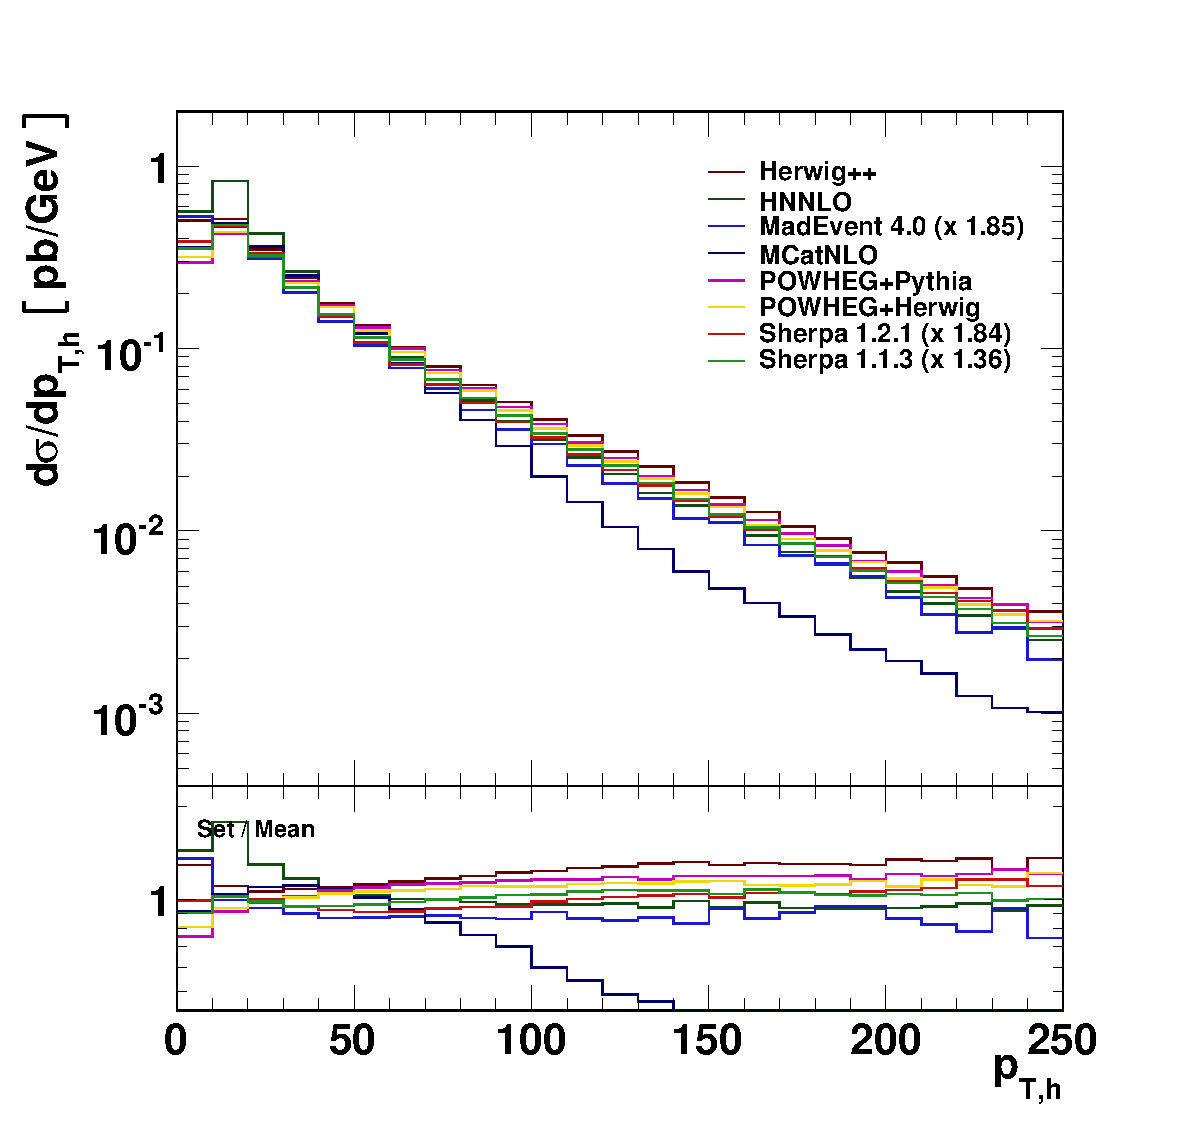
\includegraphics[width=.48\linewidth]{YRHXS_NLOMC/YRHXS_NLOMC_fig1.ps}
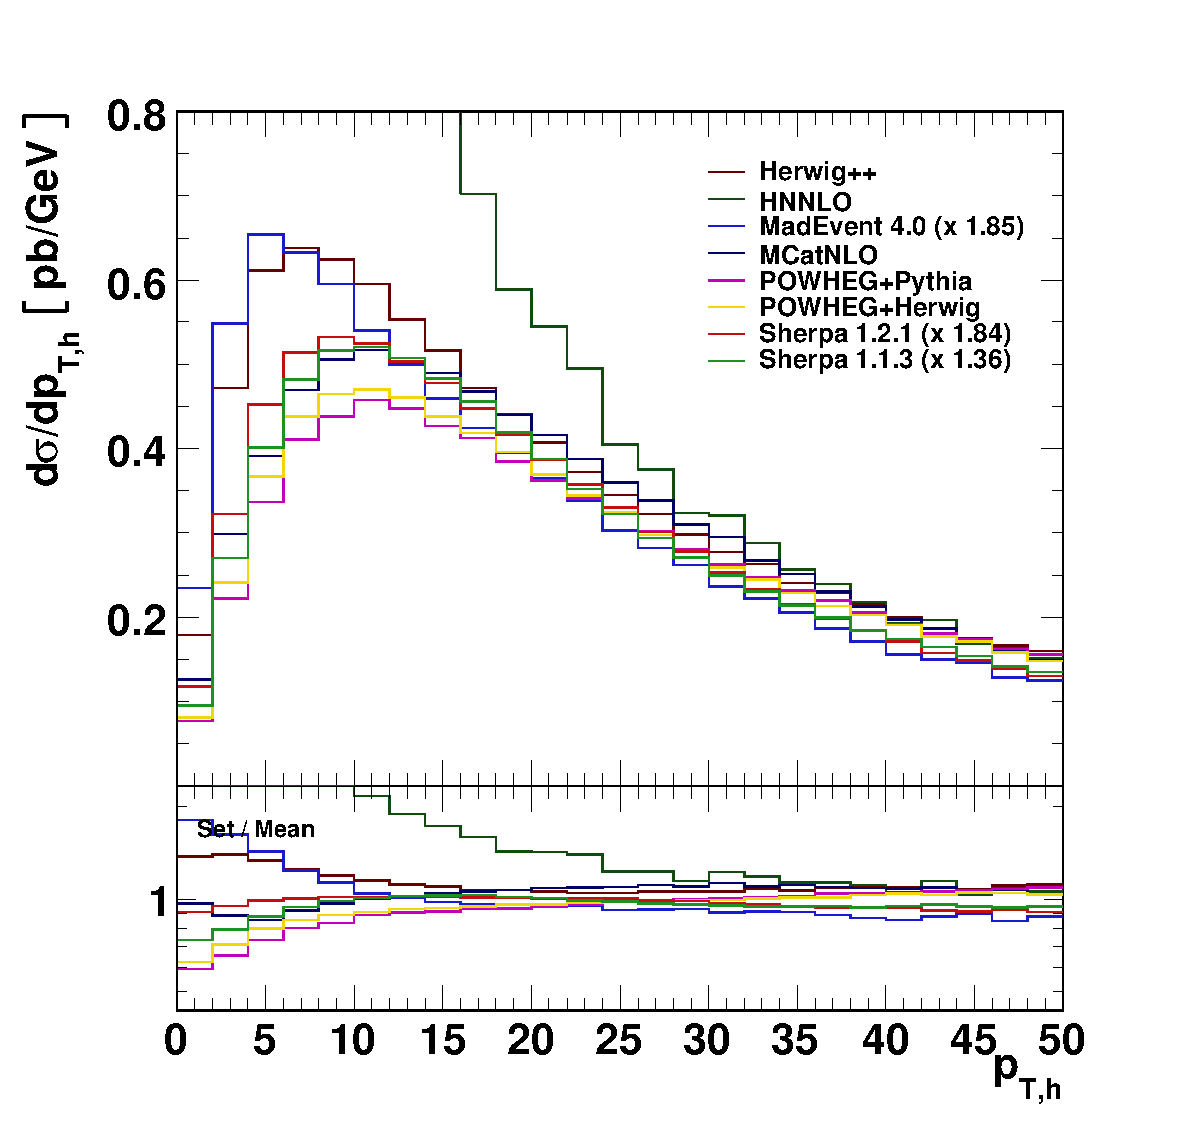
\includegraphics[width=.48\linewidth]{YRHXS_NLOMC/YRHXS_NLOMC_fig2.ps}
%\vspace*{-15pt}
\caption{Comparison of the $\pT$ spectrum of the
Higgs in various approaches, from \Bref{Butterworth:2010ym}.}
\label{fig:ptHLesHouches}
\end{figure}
In particular, the \MCatNLO{} result 
exhibits a much softer $\pT$ spectrum, for transverse
momenta above roughly one half of the Higgs-boson mass. The transverse momentum
region below $15$\UGeV\ (i.e.\ the Sudakov region) also displayed a somewhat 
different behaviour, being peaked around $5{-}6$\UGeV\ for \herwigpp{} and \MGME{}+\pythia{}
while for all the others the peak is slightly above $10$\UGeV. On the other hand,
this discrepancy cannot be considered fully conclusive, since hadronisation
effects -- although expected to be small -- were only included in the 
\MCatNLO and \POWHEG output.

In \Bref{Alioli:2008tz}, a further detailed study was carried out 
comparing results from \pythia{}, \POWHEG{}, and \MCatNLO{} with the fixed-order 
NNLO calculation, and with the NNLL resummed transverse-momentum
distribution of the Higgs boson.  
The findings of the study can be summarised in few points: 
\begin{itemize}
\item First of all, the \pythia{} (including MEC)
      distributions differ from the \POWHEG{} 
      ones by a $K$-factor that depends only mildly upon the Higgs rapidity. 
      This is explained by the fact that the first radiation in both
      is of the same accuracy, the only difference being that in \pythia{} 
      it is $B$ rather than $\bar{B}$ that appears in front of this formula.
\item This observation also clarifies why all methods but \MCatNLO{} yield 
      very similar transverse-momentum spectra.  We can understand the reason
      for this behaviour from Eq.~(\ref{eq:nlocorr1}).
      We see the reason for this: here the $K$-factor is applied to ${\cal S}$
      events only, but not to ${\cal H}$ events. These last ones populate 
      the region of $\pT$ above roughly $60$\UGeV, and 
      they are not amplified by the large $K$-factor present in Higgs 
      production.
\item The Higgs transverse-momentum distribution in \POWHEG{} shows
      very good agreement with the NNLO calculation. Again we should state 
      that the transverse-momentum spectrum of the Higgs is only computed
      at leading order in \POWHEG{} (being in fact part of the NLO correction
      to inclusive Higgs production). The presence of the full $K$-factor 
      in front of this distribution should thus be seen as an arbitrary 
      correction, trying to catch the true NNLO one. 
\item Similar observations also apply to ME+PS and \pythia{} results rescaled 
      to the full NLO cross section. It turns out, in this case, that the 
      NNLO calculation is in better agreement with these results.  It is 
      not clear whether this is a general pattern of NNLO corrections; however,
      while the same pattern is observed also in $\PW$ and $\PZ$ production
      it should be noted that these processes, being $s$-channel production
      as well are very similar to Higgs production. It would be interesting 
      to investigate whether this is also the case in processes for which 
      the NLO corrections to the production of an associated jet is also 
      known, like, for example, $\PQt\PAQt$ production.
\item In the Sudakov region the transverse-momentum distribution of \POWHEG{} 
      agrees well with the analytic NLL calculation of \Bref{Bozzi:2005wk}, 
      while the also available NNLL result is above \POWHEG{}, but with a 
      very similar shape (see \Fref{fig:HqTpwg}).
\begin{figure}[htb]
%\vspace{5pt}
\centering
\includegraphics[width=.48\linewidth]{YRHXS_NLOMC/YRHXS_NLOMC_fig3.eps}
\includegraphics[width=.48\linewidth]{YRHXS_NLOMC/YRHXS_NLOMC_fig4.eps}
%\vspace*{-15pt}
\caption{Comparison of the Higgs $\pT$ spectrum
of {\protect \POWHEG}
compared with the analytical resummed results of \Bref{Bozzi:2005wk}
(on the left), and comparison of {\protect \POWHEG} interfaced with
{\protect \pythia},  {\protect \POWHEG} interfaced with
{\protect \herwig}, {\protect \MCatNLO} and {\protect \pythia}
standalone (on the right).}
\label{fig:HqTpwg}
\end{figure}
      This can be understood as being mostly an effect 
      due to the inclusion of NNLO terms in the analytic calculation,
      which globally increases the cross section.  In the same region, 
      \MCatNLO{} and \POWHEG{}, when both interfaced to \herwig{}, give very 
      similar results.  This region is the most likely to be important when a 
      jet veto is applied, and is affected by several physical effects of 
      perturbative and non-perturbative origin. These should be studied, 
      for example, using the \POWHEG{} and ME+PS methods, preferably 
      interfaced to different shower programs.
\end{itemize}

Detailed studies comparing \MCatNLO, the NNLO, and the NNLL results
for specific Higgs decay modes have been performed in
\Bref{Stockli:2005hz}
for the $\PGg\PGg$ channel, and in 
\Bref{Anastasiou:2008ik} for the $\PW^+\PW^-$ channel.
In both cases, a good agreement is found for the acceptance correction
found using the parton-level NNLO calculation and \MCatNLO.
This is quite remarkable, especially for the $\PW^+\PW^-$, where a jet veto
is an essential ingredient to suppress the large $\PQt\PAQt$ background.
Since the NNLL result only predict the inclusive transverse-momentum
distribution of the Higgs, it is used to validate the shower Monte Carlo
results. It is found that the NLL and also the NNLL results for the Higgs
cross section below a given transverse-momentum cut match
well with the shower results (consistently with what is displayed in
\Fref{fig:HqTpwg}), and also with the NNLO result. This is understandable,
since apparently large Sudakov logarithms are important for this distribution.
The shower Monte Carlo's (\MCatNLO and \herwig) both resum these logarithms
at the NLL level, and in the NNLO result one more logarithmic term is
included in the cross section with respect to the NLO one.

Hadronization and the underlying event are both likely to affect the
efficiency of the jet veto, by adding more activity to the event.
In \Bref{Anastasiou:2008ik} these effects are also
studied using \herwig\ and {\sc JIMMY}~\cite{Butterworth:1996zw}, for both a cone and 
a $\kT$ algorithm.
The results are reported here in \Fref{fig:UEeffect}.
\begin{figure}[htb]
%\vspace{5pt}
\centering
\includegraphics[width=.48\linewidth]{YRHXS_NLOMC/YRHXS_NLOMC_fig5.ps}
\includegraphics[width=.48\linewidth]{YRHXS_NLOMC/YRHXS_NLOMC_fig6.ps}
%\vspace*{-15pt}
\caption{ %\label{fig:UEeffect}
Difference of the cross section after signal cuts including the underlying
event and the hadronization model, with respect to the partonic cross section,
from \Bref{Anastasiou:2008ik}.
The cross section is shown as a function of the jet veto for both the
SISCone and the $\kT$ clustering algorithm.}
\label{fig:UEeffect}
\end{figure}
Effects of the order of $10\%$ are found for a jet veto of $25$\UGeV,
with the hadronization and the underlying event acting in opposite directions.
It would be desirable to extend these studies using other shower and
underlying event models.

\subsubsection{VBF}

Vector-boson fusion is available in the ME+PS approach in several matrix-element-based 
generators, such as \alpgen, \MGME\ and \sherpa\ as well as in 
the \POWHEGBOX{} implementation~\cite{Nason:2009ai}.   Another \POWHEG\
implementation will be available soon also in the \herwigpp\ event generator.

At variance with the gluon-fusion process, in VBF, NLO corrections are 
very small and extra QCD radiation in general is rather suppressed\footnote{
     It should be noted that for VBF the electroweak corrections are roughly 
     as large as the QCD ones, but there is currently no attempt to include
     them into a full simulation.
}. This feature is exploited experimentally to enhance the signal over the 
background by requiring a jet veto in the central region.  Due to angular 
ordering a simple PS approach is expected to work well for VBF; in 
order to estimate uncertainties related to details of the parton shower, a 
careful study invoking ME+PS and NLO+PS could be important.  A first study 
along these lines, using ME+PS, was presented in \Bref{DelDuca:2006hk}, 
where indeed substantial agreement between parton-level predictions and those 
merged with the PS on the key observables were found.

A more recent study compared the NLO fixed-order computation with the POWHEG 
implementation interfaced to both \pythia\ and \herwig~\cite{Nason:2009ai}.  
All the most relevant distributions are compared, from the most inclusive to 
the more exclusive. On the former, good agreement with fixed-order 
computations and only mild sensitivity to shower effects is found, confirming 
the small effects due to extra radiation.  However, for the more exclusive
observables, some discrepancies showed up.  As the probably most prominent 
example for such a discrepancy consider the efficiency of the central jet 
veto compared to fixed-order LO and NLO computations.  At low transverse 
momentum, where soft-resummation effects are important, fixed-order 
calculations cannot be reliable and resummation, realised by a parton-shower 
approach, becomes mandatory.  Thus, in this case sizable differences between 
fixed-order calculations and the parton shower are expected and indeed found.  
All in all, jet-veto effects show some appreciable dependence on resummation 
and therefore on the shower algorithm, at least for low $\pT$ veto, see 
Fig.~10 of \Bref{Nason:2009ai}.  

This may deserve a further, more careful study, also including the impact of 
e.g.\ PDFs and the underlying event.  On the same footing, it would be 
interesting to further compare the effect of jet vetoes or jet azimuthal 
correlations to fixed-order calculations that include one extra jet at 
NLO~\cite{Figy:2007kv} and to top-loop-induced 
$\PH + 2\,$jets~\cite{Campbell:2010cz}.

\subsubsection{VH}
Due to its comparably simple structure, Higgs associated production
with a vector boson is available at the NLO and NNLO level; while the former 
is fully worked out, including spin correlations in the decays, such 
differential distributions in general are lacking for the latter.  In 
addition, this process is also implemented in both the \MCatNLO and the 
\POWHEG approach.  A detailed discussion of these implementations, together 
with a tuned comparison with fixed-order results at NLO accuracy is available 
in \Bref{Hamilton:2009za}.  

In addition, standard ME+PS tools such as \alpgen, \MGME, and \sherpa\ are 
also capable to simulate this process.  It should be stressed, however, that 
for searches based on the boosted-Higgs idea of~\cite{Butterworth:2008iy} the 
impact of higher-order corrections to the Higgs decay into $\PQb$~quarks and
especially the impact of hard gluon radiation off the $\PQb$'s is a
crucial ingredient.  Therefore further studies on all possible levels
would be certainly most welcome.


\subsubsection{ttH}

As of today, no public code including either, at the parton-level NLO, or 
a full simulation in the \MCatNLO or \POWHEG frameworks, is available for 
Higgs production in association with top quarks.  However, ME+PS matching is 
available in several matrix-element-based generators, such as \alpgen, 
\sherpa, and \MGME.  

However, as in VH, an accurate simulation of the Higgs decay to $\PQb\PAQb$, 
which includes extra hard radiation at the matrix element level, is 
recommended.

\subsection{Modelling the Higgs boson in scenarios beyond the
Standard Model}

Accurate simulations of Higgs production in scenarios beyond the  
Standard Model will be needed both in the identification of the 
interesting 
signatures and also in the extraction of key information, such as masses,
couplings strengths, and CP structure. As a template one can consider a  
general two-Higgs doublet model, which encompasses the much more studied 
SUSY cases and displays five scalar particles, three neutrals and one charged
pair. Other extensions to higher representations, such as triplets,  
are also often considered.

The status of the MC tools in such models is quite different from that  
outlined above for the Standard Model (SM) Higgs.  As many new physics models are now 
easily implementable in matrix-element generators such as \MGME or in \sherpa, 
ME+PS predictions are de facto available for many interesting scenarios, 
including the minimal supersymmetric SM (MSSM) or extensions such as the 
next-to-MSSM. To our knowledge, however, no 
systematic comparisons with standard PS or fixed-order NLO calculations 
have been performed.

Regarding NLO+PS the availability for cenarios beyond the
Standard Model is much more limited. There 
are, however, notable exceptions. All processes in the new physics 
scenarios that can be obtained from those in the SM by simply rescaling the 
coupling strength and masses can be easily simulated. As an example, consider
VBF and VH for SUSY neutral Higgs production, where the cross sections for the
MSSM Higgs bosons $\Ph$ and 
$\PH$ can be obtained by such a simple rescaling. 

An example where simple rescaling will not work is the case of gluon fusion 
where a $\PQb$-quark loop could give a sizable contribution in the large-$\tan\beta$ 
scenarios. In this case, the usual approach of using the Higgs-effective
theory cannot be applied, and more work is needed (and would be welcome).  In 
addition, in SUSY scenario, effects from heavy coloured states would also 
play a role.

On a similar level, new calculations may be recycled for other channels. For
example, when a $\PQt\PAQt\PH$ calculation will be available in the 
NLO+PS framework,  with a few replacements this could be easily recycled for 
$\PQb\PAQb\PH$.  Extension to include the pseudo scalar 
$\PQt\PAQt\PA$ and $\PQb\PAQb\PA$ would also be straightforward.

Charged Higgs production is another example where a dedicated calculation was 
necessary.  Currently, the most promising mechanism is via the excitation of 
a top quark, either in association ($\PQt \PH^+$, heavy $\PH^+$) or via 
its decay  
($\PQt \to \PH + \PQb$, light $\PH^+$). The first processes is available 
in \MCatNLO ~\cite{Weydert:2009vr}. For the second one, $\PQt\PAQt$ 
production is available
both in \MCatNLO and in \POWHEG{}. However, the subsequent decay 
$\PQt \to \PH + \PQb$ can only be
simulated without spin correlations and NLO corrections at present.

\subsection{Currently used tools and wish list by the experimentalists}

%\def\fortran{Fortran\xspace}
%\def\pythia{Pythia\xspace}
%\def\phojet{Phojet\xspace}
%\def\pythiasix{Pythia~6\xspace}
%\def\pythiaeight{Pythia~8\xspace}
%\def\herwig{Herwig\xspace}
%\def\herwigsix{Herwig~6\xspace}
%\def\herwigpp{Herwig\raisebox{0.1ex}{\small $++$}\xspace}
%\def\sherpa{Sherpa\xspace}
%\def\alpgen{AlpGen\xspace}
%\def\helac{HELAC\xspace}
%\def\charybdis{Charybdis\xspace}
%\def\jimmy{Jimmy\xspace}
%\def\rivet{Rivet\xspace}
%\def\rivetgun{Rivetgun\xspace}
%\def\professor{Professor\xspace}
%\def\fastjet{FastJet\xspace}
%\def\hepmc{HepMC\xspace}
%\def\agile{AGILe\xspace}
%\def\hztool{HZTool\xspace}
%\def\numpy{NumPy\xspace}
%\def\scipy{SciPy\xspace}
%\def\minuit{Minuit\xspace}
%\def\pyminuit{PyMinuit\xspace}
%\def\python{Python\xspace}
%\newcommand\POWHEG{{\tt P\scalebox{0.9}{OWHEG}}\xspace}
%\newcommand\POWHEGBOX{{\tt P\scalebox{0.9}{OWHEG} B\scalebox{0.9}{OX}}\xspace}
%\newcommand\MCatNLO{{\tt M\scalebox{0.9}{C}@N\scalebox{0.9}{LO}}\xspace}
%\newcommand\ARIADNE{{\tt A\scalebox{0.9}{RIADNE}}\xspace}
%\newcommand\ADICIC{{\tt A\scalebox{0.9}{DICIC}++}\xspace}
%\newcommand\AMEGIC{{\tt A\scalebox{0.9}{MEGIC}++}\xspace}
%\newcommand\Comix{{\tt Comix}\xspace}
%\newcommand\HNNLO{{\tt H\scalebox{0.9}{NNLO}}\xspace}
%\newcommand\MGME{{\tt M\scalebox{0.9}{AD}G\scalebox{0.9}{RAPH/}M\scalebox{0.9}{AD}E\scalebox{0.9}{VENT}}\xspace}

The experimental collaborations use a collection of publicly available tools, which are 
properly versioned, maintained, well described, and referenced.  Typically
all multi-purpose or parton-level event generators fall into this category.
A list of currently used Monte Carlo generator tools for mass production of 
fully simulated and reconstructed events is presented in Table~\ref{tab:nlomctabone}.

%%%%%%%%%%%%%%%%%%%%%%%%%%%%%%%%%%%%%%%%%%%%%%
\begin{table}[t]
\begin{center}
\caption{Combined set of Monte Carlo event generator tools currently used for mass production by the ATLAS and CMS collaborations.  Most of these tools are used by both the collaborations, few are used in one collaboration only.  The version numbers in the table represent the latest versions used but lower versions are also used in experiments due to validation and coordinated production schedules.}
\footnotesize{
\begin{tabular}{|c|c|c|c|c|} \hline
Type               &    Physics        &	Generator &	Version       &	Comments \\  
             &     processes       &	 &	      &	 \\  
\hline %------------------------------------------------------------------------------------------------------
                       &                                       &                       &                      &                       \\  
Multi-purpose & 	EW, QCD,            &      PYTHIA6   &    6.423      & Standard tune D6T  \\
LO generators     & SM Higgs,                      &	                  &	                   &   with Q2 PS,            \\
                       &   MSSM Higgs                 &                       &                      &  PS hadronization  for                      \\  
                       & SUSY, exotica                &                        &                      & MADGRAPH, ALPGEN, \\   
                       &                                      &                        &                       &and TopRex   \\  
                       &    QCD di-jet                  &   PYTHIA8      &    8.145          &                                 \\  
                       &                                      &                        &                       &                       \\  
                       &  QCD studies                 &  HERWIG6    &     6.510        &  PS hadronization  for   \\  
                       &                                       & HERWIG++  &    2.4.2          & MADGRAPH, ALPGEN,  \\  
                       &                                       &                       &                      & MC@NLO and POWHEG          \\  
                       &                                       &                       &                      & interfaced to JIMMY  \\ 
                      &                                       &                       &                      &   (V4.31) for UE/MI                     \\  
                     &                          &                       &                      &                       \\     
\hline %------------------------------------------------------------------------------------------------------
                     &                          &                       &                      &                       \\   
Dedicated  	     &  gg$\to VV$                     &  gg2ZZ,   gg2WW  &   1.0.0 &                  \\  
LO  generators       &          $\PQt\PAQt$                &   TopRex     &       4.11   &                       \\   
                     &                          &                       &                      &                       \\   
\hline %------------------------------------------------------------------------------------------------------
                     &                          &                       &                      &                       \\    
 Multi-leg         & QCD,                    &  MADGRAPH  &  4.4.13        &        \\  
  matrix-element  & Q+jets, QQ+jets,       &                        &                 &                               \\  
 LO  generators    & $\gamma$+jets, $\gamma\gamma$+jets, &   &           &                              \\  
                       &  $V$+jets, $VV$+jets, &     SHERPA        &   1.2.2          &   \\        
                       & $\PQt\PAQt$, single top, $\PZ'$  &                       &                      &                       \\  
                       &                                       &                       &                      &                       \\  
                      &    $V$+jets, $V\PQb\PAQb$,            & ALPGEN &     2.13  &  \\  
                      &    QCD, $\PQt\PAQt$          &              &                 &                                      \\  
                     &                          &                       &                      &                       \\   
\hline %------------------------------------------------------------------------------------------------------
                      &                          &                       &                      &                       \\   
NLO event      &DY, $\PW\PW$,                        & MC@NLO &   3.41/3.42      &                        \\  
generators     & $\PQt\PAQt$, single top,  &                       &                      &                      \\  
                       &    ggF Higgs                    &                      &                      &                       \\  
                       &                                       &                      &                      &                       \\  
                       & Drell--Yan, Higgs                       &  POWHEG      &                      &                       \\  
                      &                                       &                       &                      &                       \\   
\hline %--------------------------------------------------------------------------------------------------------
\end{tabular}
}
\label{tab:nlomctabone}
\end{center}
\end{table}
%%%%%%%%%%%%%%%%%%%%%%%%%%%%%%%%%%%%%%%%%%%%%%%%

%%% 
% Reference for ATLAS
% ATLAS Collab., arXiv:0901.0512 ; CERN-OPEN-2008-020 
% Title  Expected performance of the ATLAS experiment : detector, trigger and physics 
% Reference for CMS
%F. Cossutti, F. Stoeckli, CMS Collab., MC4LHC: CMS Input Document, March 2010 
% http://indico.cern.ch/getFile.py/access?resId=0&materialId=paper&confId=74601
 
For some of the inclusive-cross-section calculators, however, are just privately communicated
and, thus, are not as systematically maintained as many of the event generators tools above.  
This issue needs to be addressed to achieve a more uniform prescription on how to incorporate 
and reference these calculations properly and make the results reproducible.
On a somewhat similar footing, it is important to reference also the standard
tools in a proper manner, by indicating both version number and tune identifier,
and by making clear which tools have been interfaced with each other\footnote{
    For example, for a simulation based on \pythiasix, the exact version number
    \pythia~6.xxx {\em plus} the properly documented underlying event tune, 
    like DW, must be indicated.  Similarly, when interfaced with \alpgen,
    the results should be called ``\alpgen~2.xxx+\pythiasix.yyy~(DW)'' or 
    similar.  
}.

At the same time, flexibility of cross-section calculator tools that 
allow detailed experimental cut and efficiency analyses and the
inclusion of fully exclusive final states into their results are critical.  
It would therefore be highly desirable to turn as many NLO calculations as 
possible into hadron-level event simulations.  A possible avenue, of course, 
would be to ask the authors of the respective NLO codes to facilitate turning 
their calculations into a full-fledged simulation, through either \POWHEG{} or
\MCatNLO{} techniques.  Automation of the whole process (NLO computation and 
interface to the parton showering) is also possible.

%%% MF20101120 - included in the itemized wish-list below
%Obviously, including NLO accuracy into the Higgs boson
%decays ($H\to b\bar b$, and, maybe electroweak corrections in $H\to WW$)
%as well as covering the heavy-quark associated production of Higgs bosons
%should rank pretty high on the list of priorities.

It should be stressed, however, that it is necessary for all theoretical 
tools to be maintained and remain accessible at all times.   
A commonly agreed central code repository, such as
the Hepforge database ({\tt http://www.hepforge.org/}) would be highly 
useful for improved accessibility and maintenance. 


Based on the most immediate needs for the Higgs searches in the experiments, 
a wish list for theorists is also proposed as follows for the Higgs-signal 
MC and for background studies.
For Higgs signal MC generators, main processes that need urgent implementation are:
\begin{itemize}	
\item NLO corrections to $\PH\to \PQb\PAQb$  decay\footnote{
  An unreleased patch of HERWIG is available for NLO corrections to 
$\PH\to \PQb\PAQb$  decay.  For the experimental collaborations,  it       
 would be ideal to have this process implemented in the official 
\herwigpp\ release.
%Herwig++   
ME+PS corrections to $\PH\to \PQb\PAQb$  decay can be easily implemented 
also in \sherpa\ in which these corrections are already implemented for 
$\PQt$ decays.},
\item Finite $\Mt/\Mb$ in $\Pg\Pg\to \PH$ production  (especially relevant 
for SUSY Higgs),
\item $\Pp\Pp\to (\PQt\to \PH^+ \PQb) \PAQt$, including a treatment of  
$\PQt \to \PH^+ \PQb$ decay
with the
same level of accuracy achieved in $\PQt\to \PW+ \PQb$ in \MCatNLO{} and 
\POWHEG{},
\item $\Pp\Pp\to \PQt\PAQt \PH$ and $\Pp\Pp\to \PQb\PAQb \PH$,
\item $\Pp\Pp\to \PQb\PH$. 
\end{itemize} 

For background MC generators, main processes needed to be implemented at NLO are (listed in order of implementation complexity):
\begin{itemize}
\item $\PQq\qbar \to \PZ\PZ^*$  (now available without gamma interference),
\item $V\PQb\PAQb$,
\item $\PQt\PAQt \PQb\PAQb$, $\PQt\PAQt$+jets, and $V$+jets
In particular, $V$+jets processes are the most urgent since they have the largest expected cross section of the three.
It is however already possible to perform precise measurements of $V$+jets production with 
the LHC data and test the theoretical predictions given the expected high luminosity in 
the next year.  This will help understanding vector-boson production in association 
with jets for better understanding of the crucial background process to many Higgs search channels.
\end{itemize} 

Finally, for the optimization of the experimental Higgs searches and their interpretation, 
there are two main issues: signal and background predictions and the estimation of their 
uncertainties both inclusively and as a function of most important quantities used to 
separate signal from background in the experimental selections. 

For signal expectations, we have to rely on theoretical predictions.
It is recommended to use as much as possible all available higher-order MC generators, 
rather than using $K$-factors. 
In many cases NLO MC generators exist, as described in this section, thus there is 
no reason to use LO MC tools and apply $K$-factors NLO/LO to correct the 
LO predictions to NLO.
In some cases NNLO calculations exist for SM Higgs production ($\Pg\Pg\PH$ differential cross-section 
calculators) 
%- CITE Several groups)
, but not a full event generator. 
In this case, in collaboration with the authors, the NLO MC team will provide values of 
the re-weighting factors NNLO/NLO for the Higgs momentum and pseudo-rapidity distributions.

The NLO MC team will also provide guidelines on how to estimate the theoretical uncertainties 
on signal production predictions as a function of most important measurable quantities 
used to discriminate signal from background in the experimental analyses (based on 
the compilation of the common set of variables and cuts by the experimental collaborations).

Future work of the NLO MC team will be devoted to the following open questions: 
Can we devise methods to test the signal predictions before the signal itself is measured, 
by using similar and already measurable SM processes? 
For example, how a precisely the measurement of the $\PQt\PAQt$ cross section 
may help to 
reduce the uncertainty on Higgs production via $\Pg\Pg$ fusion (such as 
$\Pg\Pg\PH$)? 
More generally what measurable processes may serve as the benchmark and 
the validation of the signal predictions?

For background predictions, a number of processes can and will be measured with the 
data collected during the current and coming years at the LHC.  
$V$+jets and $V\PQb\PAQb$ predictions are urgent because they can be studied already with the LHC data. 
%% Vbb is going to be soon  implemented in POWHEG (by C.Oleari  and L. Reina) while V+jets needs manpower . 
For all background processes, experimentalists should review methods to measure 
these processes in some control regions where data statistics is abundant and 
to extrapolate the background predictions in some signal regions where data statistics 
is expected to be small. 
The theoretical predictions should give guidance and improve the precision of 
the extrapolated results.
For this, the NLO MC team will provide prescriptions on how to assign theoretical 
uncertainties to background predictions in the signal regions.


\subsection{Further issues and studies}
\subsubsection{Which tools to use?}
With the advent of better and more precise tools it becomes increasingly
important to understand which tool to pick for a given study, in order
to optimally use the best tools. Obviously it is very hard to find a 
solution that fits all eventualities, but we believe it is still worthwhile
to formulate a few guidelines:
\begin{itemize}
\item Never use one tool alone.\\
      Clearly, different tools have different accuracies and they may employ
      different approximations.  This in turn may lead to systematic  
      uncertainties, which can only be addressed by using different tools.
      Prime examples for this are uncertainties related to the underlying
      event or hadronisation, which involve a big amount of modelling.  While
      it is tempting to simply use only various tunes of the same generator
      it may be important to see if various models (e.g.\ \pythiaeight\ vs.\ 
      \herwigpp) lead to systematically different outcomes.  The same also 
      holds true for uncertainties related to parton showering etc.
\item Employ the accuracy dictated by your analysis:\\
      For very inclusive studies, like e.g.\ the rapidity distribution
      of the Higgs boson, NNLO accuracy is available and should be used.  
      For exclusive final states, the best accuracy available at the moment
      is given by the codes employing the \POWHEG and \MCatNLO techniques,
      which would yield NLO accuracy for relatively inclusive quantities
      such as the Higgs-boson rapidity, LO accuracy for more exclusive
      quantities such as the $\pT$ distribution of the first jet,
      and PS accuracy for all further jets.  In contrast ME+PS tools yield
      LO accuracy for all jets, as long as the corresponding MEs have been
      employed.  Thus, if an analysis relies on the correct description of 
      many jets, employing the ME+PS tools is preferred, while the NLO+PS 
      tools are the tools of choice for more inclusive quantities.  Conversely,
      this suggest that pure PS tools should typically not be used.      
\end{itemize} 

\subsubsection{Choice of parton distribution functions}
For hadron colliders, parton distribution functions (PDFs) play an important 
role in determining the outcome of theoretical predictions.  Common lore
suggests that the order of the PDFs must be consistent with the order of the 
predictions.  For leading-order predictions, LO PDFs should be used while 
for NLO predictions, NLO series of PDFs need to be used.  This simple picture,
however, is somewhat blurred by the parton showers, since they partially 
include higher-order effects, as discussed above.  

%{\em FK: I've erased the incomplete listing (commented out in the source below)
%since it seems to be Atlas-specific.}
%% For ATLAS LO 22 process ME generators, MRST2007modLo [ref-mrst07-mlo] is 
%% used while for other ME generators, such as Alpgen [ref-alpgen] and 
%% MadGraph [ref-madgraph], CTEQ6.1L [ref-cteq-61l] is used.  For \MCatNLO, 
%% CTEQ6.6 [ref-cteq-66] is used.   The \MCatNLO output is fed through HERWIG 
%% [ref-herwig] for parton showering and underlying event (UE) additions and 
%% JIMMY [ref-jimmy] for multiple interactions. In addition, the dedicated 
%% tune was done for HERWIG+JIMMY using CTEQ6.6.

This issues is further obfuscated by the often large impact the PDF has on 
the underlying event simulation.  It is therefore important to ensure that
the PDFs are used in a conscientious way -- changing a PDF without changing 
other parameters may lead to huge and unphysical effects.  Therefore, in 
order to assess PDF uncertainties by comparing apples to apples, it would be 
paramount to have at hand various tunes for the underlying event etc.


\subsubsection{Interfacing codes}
Many of the tools discussed in this section are based on interfacing a
parton-level calculation at leading (\alpgen\ and \MGME) or next-to leading 
order (\POWHEGBOX and \MCatNLO) to a full event generator that includes the 
parton showers, the underlying-event simulation, and hadronisation.  While
most likely uncritical for very inclusive observables such as cross section,
a number of issues may arise for more exclusive observables such as jet 
production, jet spectra, and jet vetoes.  Since they have not been studied 
in details, it may be worth pointing out a few of these issues: 
\begin{itemize}
\item Typically, for NLO calculations, an NLO PDF is used, and the strong 
      coupling constant of this PDF is employed, to guarantee the theoretical
      consistency of the calculation.  In a similar fashion, already on the
      tree-level choices concerning PDFs and $\alphas$ are made.  When 
      interfacing such parton-level codes with their choice of PDFs etc.\ 
      with a parton-shower code such as \pythia\ or \herwig\ in a specific 
      tune, which also includes a definition of PDFs and $\alphas$.  
      This renders the evaluation of PDF and scale uncertainties a tricky
      task, for which no prescription has been defined yet.  
\item In this context it is worth noting that for ME+PS tools, which {\em sit} 
      on a full event generator, the merging algorithm often employs the
      Sudakov form factors of the underlying parton shower.  This may then
      lead to the counter-intuitive effect that a {\em harder} tune for the
      parton shower yields softer jets when interfaced with parton-level
      MEs.
\item As discussed above, quantities such as the central-jet veto in VBF
      depend on resummation properties -- typically the realm of the parton 
      showers in the simulations currently used by experimenters.  It would
      therefore be worthwhile to check for these effects in different
      interfaced codes, including the impact of the underlying event in 
      a more complete fashion.  
\end{itemize}

\subsection{Conclusions}

As we are entering the LHC running phase, we have available several very 
accurate {\em theoretical-style} predictions in the form of parton-level integrators that 
can output histograms for any IR-safe observable.  On the other hand, 
Monte Carlo event generators with NLO accuracy are now (or will be soon)  
available for all the relevant Higgs production processes. A systematic 
comparison between various implementations, PS programs and fixed or 
improved {\em theoretical-style} calculations is now possible. 

In this brief note we have listed the available tools and also given an 
example (taken from \Bref{Butterworth:2010ym}) on how such comparisons 
can be made.

The tunes for the various Monte Carlos need to be re-established as 
components relevant to assess, for instance, systematic uncertainties due to
PDFs.  We expect this to be a continuous process as the implemented order of 
calculations change and new codes and physics processes become available.  
Finally, it is important to establish 
\begin{itemize}
\item a consistent set of Standard Model parameters for MC tools  
      (the MC4LHC group is to provide a suggested set of these parameters),
\item a consistent and complete way to reference the tools used,
\item a common code repository,
\item procedures to cross compare and validate different codes and 
      implementations,
\item procedures to assess systematic uncertainties of the theoretical 
      predictions and simulations.  
\end{itemize}


\clearpage
